\documentclass[12pt, a4paper]{article} 

\usepackage[utf8]{inputenc}


\usepackage{geometry} % to change the page dimensions
\geometry{a4paper} % or letterpaper (US) or a5paper or....

\usepackage{graphicx} % support the \includegraphics command and options

\usepackage{booktabs} % for much better looking tables
\usepackage{array} % for better arrays (eg matrices) in maths
\usepackage{paralist} % very flexible & customisable lists (eg. enumerate/itemize, etc.)
\usepackage{verbatim} % adds environment for commenting out blocks of text & for better verbatim
\usepackage{subfig} % make it possible to include more than one captioned figure/table in a single float
% These packages are all incorporated in the memoir class to one degree or another...



\usepackage{amsmath, amssymb}% for mathematical symbols
\usepackage[colorlinks=true,linkcolor=black]{hyperref} % for hyperreferences with black color
%\usepackage[T1]{fontenc} % Uncomment for norwegian document
%\usepackage[norsk]{babel} %

%%% HEADERS & FOOTERS
\usepackage{fancyhdr} % This should be set AFTER setting up the page geometry
\pagestyle{fancy} % options: empty , plain , fancy
\renewcommand{\headrulewidth}{0pt} % customise the layout...
\lhead{}\chead{}\rhead{}
\lfoot{}\cfoot{\thepage}\rfoot{}

%%% SECTION TITLE APPEARANCE
\usepackage{sectsty}
\allsectionsfont{\sffamily\mdseries\upshape} % (See the fntguide.pdf for font help)
% (This matches ConTeXt defaults)

%%% ToC (table of contents) APPEARANCE
\usepackage[nottoc,notlof,notlot]{tocbibind} % Put the bibliography in the ToC
\usepackage[titles,subfigure]{tocloft} % Alter the style of the Table of Contents
\renewcommand{\cftsecfont}{\rmfamily\mdseries\upshape}
\renewcommand{\cftsecpagefont}{\rmfamily\mdseries\upshape} % No bold!



%%% END Article customizations

%%% The "real" document content comes below...

\title{Specialization project}
\author{Hong-Dang Lam}
%\date{} % Activate to display a given date or no date (if empty),
         % otherwise the current date is printed 

\begin{document}
\pagenumbering{gobble}
\maketitle
\pagenumbering{roman}
\newpage
\begin{abstract}

Abstract

\end{abstract}

\newpage
\tableofcontents
\newpage
\pagenumbering{arabic}
%1 introduction
\section{introduction}
insert introduction here

%2 related works
\section{Background}
Background introduction

\subsection{Swarming}
Swarm, swarming, swarm intelligence, swarm optimization or swarm robotics are terms used for simple (preferably cheap) robots which can only do simple tasks. However the power of these robots lies in the numbers. The robots might not be able to do an advanced task alone, but together they might be able complete advanced tasks. For instance, one robot might not be able to push a heavy box by itself, but with the help of other robots they might be able to push the box.
Each robot are allowed to communicate with each other, but they do not need to communicate. There are no centralized controller that controls the robot, each one needs to find out what it needs to do by itself or by communicating with the other robots. The idea behind these simple cheap robots are that they can easily be mass produced, interchangeable, modularized and disposable. If one robot is malfunctioning or broken, it would not affect the rest of the swarm. It is therefore no single point of failure in a swarm, and the system is very scalable because robots can easily be added to the system.
Swarm robotics are often very computer efficient, because they each have their own processor. This reduces the computational overhead. 

\subsection{Boids}
In 1986, Craig W. Reynolds created something called Boids, which stands for \textbf{B}ird-\textbf{oid} object\textbf{s}. Boids are particles that would behave like birds, they would try to flock and fly together without colliding. This was done by using 3 simple behaviors;
\begin{description}
    \item[Separation]
        Each individual will steer away from the other individual if they were too close to each other. This ensure that they do not collide with their neighbors.
    \item[Alignment]
        In a neighborhood (for instance a radius around the individual or the $X$ nearest individuals) find the average angle of the neighborhood and align itself so its angle matches the average angle of the neighborhood.
    \item[Cohesion]
        Steer towards the average position of the other individuals in your neighborhood. This makes the Boids stay in the flock.
\end{description}
\begin{figure}[H]
    \centering
    \subfloat[Separation ]{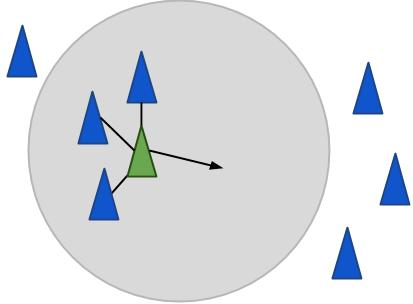
\includegraphics[width=0.3\textwidth]{images/boid_separation.jpg}}
    \hfill
    \subfloat[Alignment ]{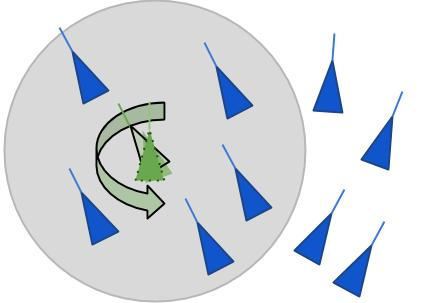
\includegraphics[width=0.3\textwidth]{images/boid_alignment1.jpg}}
    \hfill
    \subfloat[Cohesion ]{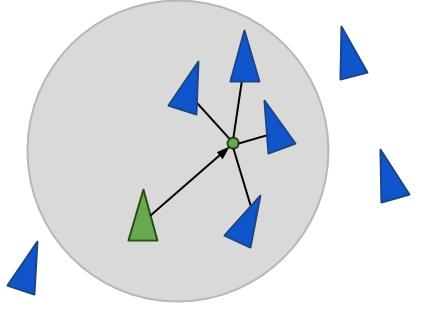
\includegraphics[width=0.3\textwidth]{images/boid_cohesion.jpg}}
            \caption[Boids behavior]{The three behaviors of the Boids}
            \label{fig:boidbehavior}
\end{figure}

The three behavior is per individual Boid, which means that each particle/Boid has to calculate where they are going to fly by checking all the other Boids position and rotation and then act accordingly. Which makes this algorithm $ O(n^2)$ for every frame. 
Reynolds have tried to make the algorithm less computational intensive by putting the Boids into grids with Spatial Hashing. An example of could be to put all the Boids that has a position $0<x<1$ and $0<y<1$ on the lower left grid, and the ones that has a $1<x<2$ in the next position etc. Using this grid, each Boids in a cell only needs to take the adjacent grids into consideration when checking their neighborhood. 
\begin{figure}[h!]
    \centering
    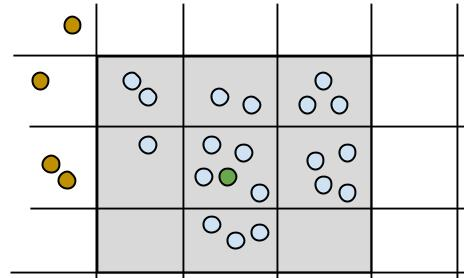
\includegraphics[width=0.8\linewidth]{images/boid_spatialhash}
    \caption{Boids in grids using spatial hash} \label{fig:spatialhash}
\end{figure}
As illustrated in the figure, the green Boid only needs to check the gray Boids that surrounds its own cell, it does not need to check the rotation and position of the orange/brown Boids outside of the gray box, because they are too far away to be considered a part of its neighborhood.

In another paper a different technique were used to optimize 3D swarms, a method using neighborhood grids.\\

Other optimization has been made as well, like the neighborhood grid.
Each Boids to cell ratio would be 1 to 1, that is for every cell, there would be at max 1 Boid. Each Boid would have their respective cell based on their position in space, for instance a Boid with low $x$-value would be on the left of a Boid with higher $x$-value, and Boids who are closer to each other in geometric space would be stored closer to each other in the grid. To obtain this, the Boids needed to be sorted. Odd Even sort and Bitonic sort were used as the sorting algorithm.\\
Of the two sorting algorithm, Odd Even sort was faster, but not very precise. More than 10\% of the entities were placed in the wrong cell. The paper did an odd even sort algorithm for each axis, that is one odd even sort for x, y and z in paralell.\\
Bitonic Sort on the other hand was slower, but a lot more precise. Less than 1\% of the entities were placed in wrong cell. The reason for placing a Boid in the wrong cell is due to way the sorting works, it sorts all the entities in one axis first, then a second axis and then the third last axis. For instance sorting on $x$-values first, for the $y$-values, then the $z$-values. When swapping one of the latter axises it might mess up the sorting of one of the other axises.

After the Boids were placed in their corresponding grid, the work could be distributed to the GPU which would calculate where each Boids' new location and rotation would be based on their adjacent neighbor depending on the Moore radius.
The paper tried to vary the number of Boids from 1,000 to 1,000,000 and they had 4 types of Boids. The same types of Boids would try to flock with each other while different types of Boids would try to avoid each other.
They were able to see a speedup compared to the spatial hashing method used by Reynolds, but the Boids were not rendered as a bird or an object, only as a primitive shape. They didn't mention if they tried to add non moving obstacles in their test. Due to the high percentage of Boids being placed in the wrong cell when using odd even sort, a lot of Boids would crash into their neighbor during the test run. However using the neighborhood grid method on GPU, real time simulation of 1 million Boids were possible (6-8 fps).\\

In the paper "steering behaviors for autonomous character" Reynold discusses that an autonomous character, which is a type of autonomous agent are agents that have some ability to improvise their actions. That means that these agents do not have their actions scripted in advance.
These autonomous agents can have various 
in another paper he discussed various behaviours for autonomous steering, like seek, chase, flee etc.




In the paper named "not bumping into things" W. Reynolds discusses how to perform obstacle avoidance, that is obstacles that are placed in the environment which is not a boid. These obstacles are usually static, that is non moving obstacles. He starts out with the idea of a forcefield around the obstacle which he calls the \textit{steer away from surface} approach. The idea is to have every obstacle emit a forcefield around itself which pushed the boids away. For instance if a boid is flying toward an obstacle, the obstacle would push the boid to one side of itself. However this force field method would not work if the boid flew straight into an obstacle, because the forcefield force would be straight opposite of the direction the boid is flying thus making the boid deaccelerate until it stopped.
The next obstacle avoidance technique Reynold discussed is the curb feeler technique or steer along the wall technique. The idea is to have a feeler that would detect an obstacle before the boid would crash into it, then turn the boid away from the obstacle. This can be compared to walking down a dark alleyway where you'll reach your hand out to feel the walls around you and navigates through the alleywall just by feeling the wall(s).
The last technique for navigating and avoiding obstacles discussed in this paper was image processing. Images could processed in real time to a grayscale image where white would signify an obstacle. The algorithm would start with the center of the image, if this was a white pixel it would start to search outwards in a spiral to find either a gray pixel or a black one and then turn the boid in this direction. This could also be combined with a \textit{Z-buffer image} which gives us a map of the distances to obstacles that lies in front of the boid, this z-buffer iamge can be obtained by radar, sonar or similar technology. One interesting way of using the Z-buffer image is to implement a "steer towards the longest clear path". However using this technique without any form of planning or learning might lead the boid into a local cavity which might be a dead end.

In the paper Distributed physics-based control of swarms of vehicles by W. Spears and D. Spears a self emergent system is formed using simple attractive and repulsion force for each particle. The idea behind their system was to create an artificial physics framework (AP) that would simulate a physical system. In their paper they had the particles attract other particles that were farther away than distance \textit{r} and a repulsive force is applied if the particles are closer than distance \textit{r}. This leads to the particles always being at distance \textit{r} from each other which will form a hexagonal lattice. They also tried out making patterns, but had to introduce a concept of spin; each particle were either spin "down" or spin "up". Opposite spins would attract each other if the distance was greater than \textit{r} and repel each other if the distance is less than \textit{r}. If the particles had opposite spin the distance would be $\sqrt{2}r$. This means that all the vertical particles would be alternating between spin up and spin down, the same goes for the particles in the horizontal space. The diagonal particles on the other hand will have the same spins as their diagonal neighbors.

In the paper "V-like formation in flocks of artificial birds" by A. Nathan and V. Barbosa bird flocking is discussed. They ran a simulation that where each bird individual had 3 simple rules: 
\begin{itemize}
    \item Coalescing rule \\
        The birds should try to seek the proximity of the nearest bird.
    \item Gap-seeking rule \\
        If rule 1, the coalescing rule is not applicable anymore the bird should find a position with unobstructed view -  that is, the bird should be able to see in front of it without anything being in the way.
    \item Stationing rule \\
        Try to stay in place.
\end{itemize}
These rules would make sure that the birds were able to flock and form different shapes. The only thing that was common between the different runs in this paper was that the bird behind would be a little bit behind and slightly left or right of the bird in front (following rule \#2). A lot of different shapes was obtained during the runs, the birds flocked and formed a V-shape, a diagonal line, an inverted V-shape etc.

\subsection{Family bird: A heterogenous simulated flock}
This paper says that bird flocks and fish schools seems to be very complex, but the mechanics are very simple as illustrated by Reynold. Only a few simple rules will create flocks that flock together and splits up to avoid obstacles. These flocks are not spectacular or mind blowing compared to the flocks found in nature, due to the rigid motion of each individual. To tackle the artificialness of each individual, Heppner introduced randomness to the motion of the individuals, defending it by saying that these randomness simulates wind gust, random obstacles and other factors. 
However the authors of this paper does not agree with this approach because wind gusts will affect the whole flock, not just a random single individual at random. Even with these randomness added, the flock still does not seem lifelike enough compared to their counterpart found in nature. The reason for the lack of breathtaking in these flocking algorithms are that the individuals all have the same characteristics. In nature each individual will have different size, age, form and shape. 
Usually in flocking algorithms, each individual takes into account where all the other entities are and then act accordingly. In nature, each individual might have limited information about the flock, it might only be able to gain so much from its vision due to other flock members being occluded or not able to hear some of the other individuals due to noise or other factors.
This paper runs a simulation with different types of bird , where social relations are a factor and individuals might be solitary or social. Social individuals are entities who would like to stay close to members of its own social group, for instance a social dove will want to stay with other doves. Solitary individuals on the other hand does not care about staying with its own flock and might drift to another flock. For instance a solitary dove might fly amongst hawks or other types of birds. A flock in this paper are defined as a group where the individuals affect each other in the same group. The simulation they ran varied between all solitary birds to 4 types of different social birds.

\subsection{Particle Swarm Optimization}
Swarms has a lot of potential, not necessary only on robotics but swarms can be used to optimize problem, hence the name particle swarm optimization (PSO). PSOs are used to solve problems where optimization are needed. The idea behind PSOs are to have a swarm of particles spawn at random positions in the search space, and then let them fly around searching for solutions. Each particle will know the best solution it have found so far, and the best solution that is found globally. In some PSO implementations a local best found solution is also known amongst the individual. This local best solution is the best solution amongst a subgroup of individuals and can change for a particle depending on the position of the particle.

\subsection{Other swarming animals}
\subsubsection{fishes}
In this paper Xiaoyuan Tu explains how fishes form schools and how different intentions make the fish behave the way they do. He starts out with explaining how a fish and how the simulator is constructed, the math behind it and how the motor controllers work. For the simulation there's different types of fishes, some of them are predators and some of them are preys. The name explains itself, but to be clear, predators are larger fishes which tries to eat other smaller preys. Each fish has a 300 degrees, where it can see in front of it and has a blind spot directly behind it. 
The range of the vision is also limited and might be occluded by other objects. Each fish has a intention generator, which basically is a flowchart of what the fish needs to do. The prey and predator fish have different intention generators. The predators do not get preyed upon, and thus does not need to look out for other predators, therefore are the intentions of escaping, mating and schooling with other fishes of the same species are disabled. The reason for disabling mating is because there's no need for new predator fishes because they don't die in this simulation. They also don't need to school with other predators because they are not in danger, and don't need the extra survivability.\\
Whenever a predator sees a prey it will chase the prey if the cost of reaching it is minimal, if it's too much, it will not bother chasing. \\
Preys on the hand needs the extra survivability, and will try to school with the other fishes if it detects a predator nearby. Each fish will then try to stay a certain distance from each other, which is roughly on body length in distance. Then the fishes will try to adjust its speed and direction so it matches the other members. When this school of fish encounter an obstacle, they individual fishes will try to avoid this obstacle, this might lead to the school splitting up and rejoining after they have avoided the obstacle. \\
A third type of fish introduced here are the pacifists fish. This one differs from the other two type in that the intention of mating is activated while escaping and schooling are deactivated.
The paper describes that there are male and female fishes, and the two behavior which can occur when the fishes start to mate. A behavior named \textit{nuzzling} where the male fish seeks the female and nudges her abdomen until she's ready to spawn, and \textit{spawning ascent} where the female swims repeatedly to the surface while releases gametes. The paper also describes in detail how the fishes select potential partners and how they try to impress each other for mating purposes.

\subsubsection{Ant swarms/colonies}
Ant swarms behaves differently than other types of swarms, ants do not try to form formations for survival in the same way that birds and fishes do. Ant swarming are mostly about their foraging behavior, that is how they find food for their colony. Each ants' goal is the survival of the colony rather than the survival of each individual. When ants tries to find food, they scatter the area by walking in random manner. While exploring the ants leave behind a chemical on the ground, a so called pheromone that the other ants will be able to feel/smell. This pheromone will slowly but surely dissipate. Whenever the explorer ant find a food source, it will evaluate the quality of the food before returning to the anthill. During the return trip, pheromones are reapplied to the path, but the amount is adjusted based on the evaluation of the food, better food will yield higher pheromone. This method will ensure that the rest of the ants will take the shortest path from the anthill to the food.
%3 something
\section{ChIRP. Robot}
The ChIRP (CHeap and Interchangable Robotic platform) robot is a robot developed by the CRAB lab, which is part of the artificial intelligence group at the Department of Computer and Information Science (IDI) at the Norwegian University of Science And Technology (NTNU).
The purpose behind the development of the ChIRP robot is to research subsymbolic AI, wether it is swarming or evolution.
The robots' schema and source code are all open source and can be found at chirp.idi.ntnu.no. The robots' consist of a printed circuit board (PCB), 2 motors on each side with 2 wheels.
Modules like LED lights and various sensors can be soldered on the PCB thus the robots' are easily modifiable, and the robots can have multiple layers with different sensors so it's not limited to have only light sensors or IR sensors. The standard ChIRP robot comes with 8 infrared-LEDs and 8 infrared receivers. These can be used to measure distance by emitting the IR light and measure how much is reflected back into the receiver. There are 2 Shift registers ICs on top of the PCB, these shift registers handles the values found by the IR receivers and converts them to a short (the datatype, 16 bit int) so the arduino micro inside the ChIRP doesn't need to handle everyting. This is due to the limited processor power of the arduino micro which has a ATmega32u4 processor with 16 MHz clock speed and 32 KB flash memory. Arduino micro has 20 digital inpput/output (I/O) pins in which 7 of them are PWM, and 12 analog input pins. Inside the robot there's an ATtiny as well that helps the Arduino control the motors.

The ChIRPs are powered by a 3.7volts 2500mAh battery which lasts for 4.5 hours if they are running continously, and it takes 4 hours to recharge.

- All code and schemes are available on chirp.idi.ntnu.no
- PCB (printed circuit board)
- Wheels
- 2 motors
- 8 infrared emitters and receivers used for distance measuring.
- Arduino Micro microcontroller.
- Atmel chips to reduce computing on the arduino
- Modules can be added as needed.
- Blueetotth module.
- Other micropchips can be used instead.
- Battery lasts for 4.5 hours, 4 hours to charge.


\section{Traffic Sim, preproject}
The traffic simulator is a project for Statens Vegvesenet Teknologidagene in Trondheim where the ChIRP Robots was used to demonstrate platooning. 
The idea of platooning is to use an autonomous system (either global system or each individual communicates with each other) to control the vehicles, for instance cars, trucks etc. as one unit thus increasing the flow of traffic.
This leads to less air resistance and the cars will be able to cross an intersection much faster.

The whole system used a webcam with OpenCV to track the robots, all the robots were equiped with a bluetooth module and 2 circular post-it notes which was light green and pink. The camera was able to detect these post-it notes and track the position and rotation of each robot. This information was then sent to the simulation written in Java via UDP.
The simulation then calculated where the robot needed to go, set the speed for each wheel and sent the commands to the robot using the bluetooth COM-port.

The java simulation was first implemented by Magnus Hu using a game framework called Lightweight Java Game Library (LWJGL) to render everything on screen. We decided to change the framework from LWJGL to Slick2D. Slick2D is a 2D java game library which uses tools and utilities wrapped around LWJGL, which means that it can do everything LWJGL can do, but also has higher abstraction. Slick2D lets us render shapes (circles, squares) without having to specify each point and line of the shape manually.
The track used in the simulation consisted of 24 points (a point as in a point in space) laid out in a 8-shaped layout, where the center intersection is made up of 2 points.
Before running the OpenCV software and the java simulation both application needs to set a configuration parameter of how many robots are to be tracked/run. Our demo at teknologidagene used 4 robots because we only had 4 bluetooth modules. The bluetooth modules had to be connected and added as a COM port before running the simulation or else it wouldn't know where to send the commands. When starting both the OpenCV camera tracking software and the simulation, coordinates along with the rotation of each robot. At this point in time, the simulation doesn't know which coordinate and rotation (robot) belongs to which bluetoot COM port, for each robot the simulation does:
\begin{itemize}
    \item checks the angle of all the robots
    \item sends a rotate command to the bluetooth COM port, which makes a robot rotate approximately 90$^{\circ}$.
    \item checks the angle of all the robots, finds out which one has rotated the most, saves this COM port to the robot which have rotated the most
    \item rotates the robot back to the original orientation
\end{itemize}
The reason for rotating the robot back to the original orientation is because we always laid the robot out in the map facing forward, which was easier to implement instead of implementing a lot of code to ensure that the robot would face forward if it started out in the wrong direction.
Each robot will now have a COM port given that the COM port didn't time out on initiation, in which we had to restart the whole simulation program to reconnect to the COM port.
The simulation then calculates the robot's nearest point on the track, and sets the target point of the robot to be the next one, this is incase the nearest point is behind the robot. After the simulation found out where the robot should move to, it calculate which way the robot needed to rotate and which speed it should have. The speed and the amount of needed rotation ($\Delta angle$) is then converted to <"two motors"> which is sent as a byte array of 4 elements to the robot's bluetooth module. An example of the byte array could be "l40r50" which means that the right motor would drive a little bit faster than the left one thus turning the robot to the left.
If we used a capital 'L' or 'R' in the byte array instead, the wheel would turn backwards instead, however we don't use that in the simulation at all except for turning the robot in the beginning when it tries to assign the COM port to the correct robot.

The simulator creates a box in front of each robot that will be used to find out whether the robot has a robot in front of it or not. If there's a robot in front (that is inside the front box) then the simulator will check if platooning is on or not. If platooning mode is on, the robot will try to keep the same speed as the robot in front of it. At least it's not allowed to have higher speed than the robot in front of it, or else it will crash into it. If platooning mode is off, then the robot will try to keep a 3 second distance from the robot in front, that is the robot will try to keep the robot in front of it outside the detection box. The robot is considered as reaching a target if the robot's center is 20 pixels away from the target, and the next point will be assigned as the new target for the robot.
In the middle of the map, at the intersection there is a red light at the top, north side or at the right, east side of the intersection. This redd light will be alternating between these two positions depending on the user. 

\end{document}
